\documentclass{amsart}
\usepackage[margin=1in]{geometry}
\usepackage{graphicx}

\begin{document}
\title{Automatic drainage system delineation for ice sheets}
\author{Constantine Khroulev}
\date{\today}
\maketitle

\section{Introduction}
\label{sec:introduction}
Drainage basin boundaries are useful both for accounting and regional modeling.
Manual delineation is arguably the most accurate but laborious method \cite{zwally2012}.

Measured surface velocities such as in \cite{joughin2010greenland}, if
available, provide a wealth of information for basin delineation.
Unfortunately, in many cases the data coverage is too poor to provide continuous
basin boundaries.

To avoid this issue, we assume that ice flow down the surface gradient.  This
assumption is compatible with the shallow ice approximation (SIA) which describes ice
flow at the biggest scales.  Also, though the SIA is likely to be a poor description
of the flow in the fastest parts of an outlet glacier, the SIA, and the assumption
we make about flow being down the surface gradient, are appropriate along the
boundaries of the basins we are trying to delineate.

This basin delineation has been done before for the purpose of ice dynamics.
For example, Figure 1 in \cite{Joughinetal2008JGR} shows such a drainage
(``catchment'') basin, delineated for the purpose of identifying which ice flows
to the Jakobshavn calving front.  Furthermore, a drainage basin delineation tool
for ice sheets using \textsc{Matlab}'s \texttt{stream2} function developed by
D.~Dellagiustina for use with PISM \cite{DellaGiustina2011}.  The current
document is an update to open-source and free tools, as well as a re-analysis
of the method.

Ice drainage basins computed with this assumption correspond to supra-glacial
water drainage basins, and watershed delineation is a standard procedure in
hydrological modeling. Standard hydrological flow routing algorithms
\cite{lea1992aspect,jenson1988extracting,costa1994digital} do not perform well
in areas of low relief and are sensitive to grid resolution. Recent work
addressing this issue
\cite{schwanghart2010topotoolbox,seibert2007new,liang2000general,tarboton1997new}
improves delineation results, but issues related to low relief remain.

\section{The method}
\label{sec:method}

\subsection{Continuous model of a DEM}
\label{sec:continuous-model-dem}

The main idea is to use a continuous model of a DEM instead of raster-based methods.

Here we use a piecewise-bilinear interpolation of a DEM on a regular Cartesian grid.

\begin{figure}[h]
  \centering
  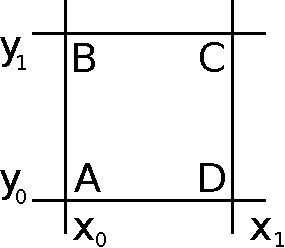
\includegraphics[width=1in]{cell.pdf}
  \caption{A DEM cell}
  \label{fig:cell}
\end{figure}

Let $A$ be the surface elevation at $(x_{1},y_{1})$, $B$ the surface elevation
at $(x_{1}, y_{2})$, etc (see Figure \ref{fig:cell}). Then on each cell (see Figure
\ref{fig:cell}) the surface elevation is given by
\begin{eqnarray}
  \label{eq:1}
  h(x,y) &=& (1-\alpha)(1-\beta)A + (1-\alpha)\beta B + \alpha\beta C +
  \alpha(1-\beta)D,\\
  \alpha(x) &=& \frac{x-x_{1}}{x_{2}-x_{1}} = \frac{x-x_{1}}{\Delta x},\\
  \beta(y) &=& \frac{y-y_{1}}{y_{2}-y_{1}} = \frac{y-y_{1}}{\Delta y}.
\end{eqnarray}

Differentiating $h(x,y)$ we get
\begin{eqnarray}
  \label{eq:2}
  \frac{\partial h}{\partial x}(x,y) &=& \frac{1}{\Delta x}(D-A) + (y-y_{1})
  \gamma,\\
  \frac{\partial h}{\partial y}(x,y) &=& \frac{1}{\Delta y}(B-A) + (x-x_{1})
  \gamma,\\
  \gamma &=& \frac{1}{\Delta x \Delta y}(A + C - B - D).
\end{eqnarray}

\section{Gradient flow}
\label{sec:gradient-flow}

To model the gradient flow originating from a grid cell we are solving the system

\begin{eqnarray}
  \label{eq:3}
  \frac{\partial x}{\partial t}(t) &=& -\frac{\partial h}{\partial x},\\
  \frac{\partial y}{\partial t}(t) &=& -\frac{\partial h}{\partial y}\\
\end{eqnarray}
with $h_{x}$ and $h_{y}$ given in \eqref{eq:2}.

Note that this system can be written as $\dot X(t) = MX + N$ with
$M =
\left[\begin{matrix}
  0 & -\gamma\\
-\gamma & 0
\end{matrix}\right]$.
The eigenvalues of $M$ are $\pm \gamma$, so this system is not stiff regardless
of the values of $A$, $B$, $C$, and $D$. Also, solutions of \eqref{eq:3} $\dot
X(t) = MX$ within the cell are hyperbolas, suggesting that a streamline $(x(t),
y(t))$ entering a cell will almost surely exit --- with the exception of
unlucky streamlines passing directly through the saddle. This is not a concern
in a practical setup, though.

\section{The algorithm}
\label{sec:algorithm}

FIXME

\section{References}
\label{sec:references}

\bibliography{references}
\bibliographystyle{siam}

\end{document}

% LocalWords: LocalWords bilinear Khroulev Joughin Zwally hydrological
